\documentclass[tikz,border=5pt]{standalone}
% Shared visual grammar: role fills, dark connectors, and 7-point typography.
% Build each standalone figure from this directory. No external images required.
\pdfinfoomitdate=1
\pdftrailerid{}
\usepackage[T1]{fontenc}
\usepackage{helvet}
\renewcommand{\familydefault}{\sfdefault}
\usepackage{amsmath,amssymb}
\hyphenpenalty=10000
\exhyphenpenalty=10000
\usetikzlibrary{arrows.meta,calc,fit,positioning,decorations.pathreplacing,backgrounds}
\definecolor{ink}{HTML}{172B3A}
\definecolor{muted}{HTML}{586D85}
\definecolor{datafill}{HTML}{F1F5F9}
\definecolor{dataline}{HTML}{62748E}
\definecolor{modelfill}{HTML}{E5E9FF}
\definecolor{modelline}{HTML}{7887C7}
\definecolor{llmfill}{HTML}{FFE4E8}
\definecolor{llmline}{HTML}{E68494}
\definecolor{truthfill}{HTML}{D0FAE5}
\definecolor{truthline}{HTML}{35A782}
\newcommand{\seven}{\fontsize{7}{8.5}\selectfont}
\tikzset{
 every node/.append style={font=\seven,text=ink,align=center},
 box/.style={draw=dataline,fill=white,rounded corners=3pt,line width=.65pt,inner sep=5pt,minimum height=8mm},
 data/.style={box,fill=datafill},
 model/.style={box,draw=modelline,fill=modelfill},
 llm/.style={box,draw=llmline,fill=llmfill},
 truth/.style={box,draw=truthline,fill=truthfill},
 title/.style={font=\seven\bfseries,inner sep=1pt},
 word/.style={text=muted,inner sep=1pt,align=center},
 label/.style={fill=white,inner xsep=2pt,inner ysep=1pt,text=muted},
 flow/.style={-{Stealth[length=2.4mm,width=1.9mm]},draw=ink,line width=1.2pt,shorten >=1.5pt},
 branch/.style={-{Stealth[length=2mm,width=1.6mm]},draw=ink,line width=.9pt,shorten >=1pt},
 route/.style={draw=ink,line width=1.2pt},
 update/.style={-{Stealth[length=2.2mm,width=1.7mm]},draw=modelline,line width=1pt,dash pattern=on 3pt off 2pt,shorten >=1.5pt},
 boundary/.style={draw=dataline,dash pattern=on 3pt off 2pt,rounded corners=3pt,line width=.6pt},
 chip/.style={minimum height=4mm,inner xsep=3pt,inner ysep=1.5pt,rounded corners=2pt},
}
% Optional role key. Anchor at the center of an uncluttered final row.
\newcommand{\rolekey}[2]{
 \node[word,anchor=east] at (#1-6.6,#2) {\textit{Key}};
 \node[data,chip] at (#1-5.2,#2) {records / data};
 \node[model,chip] at (#1-1.9,#2) {learned model / policy};
 \node[llm,chip] at (#1+1.65,#2) {LLM signal};
 \node[truth,chip] at (#1+4.95,#2) {labels / evaluation};
}

\newcommand{\introfont}{\fontsize{9}{10.8}\selectfont}
\newcommand{\introhead}[1]{{\fontsize{10}{12}\selectfont\bfseries #1}}
\begin{document}
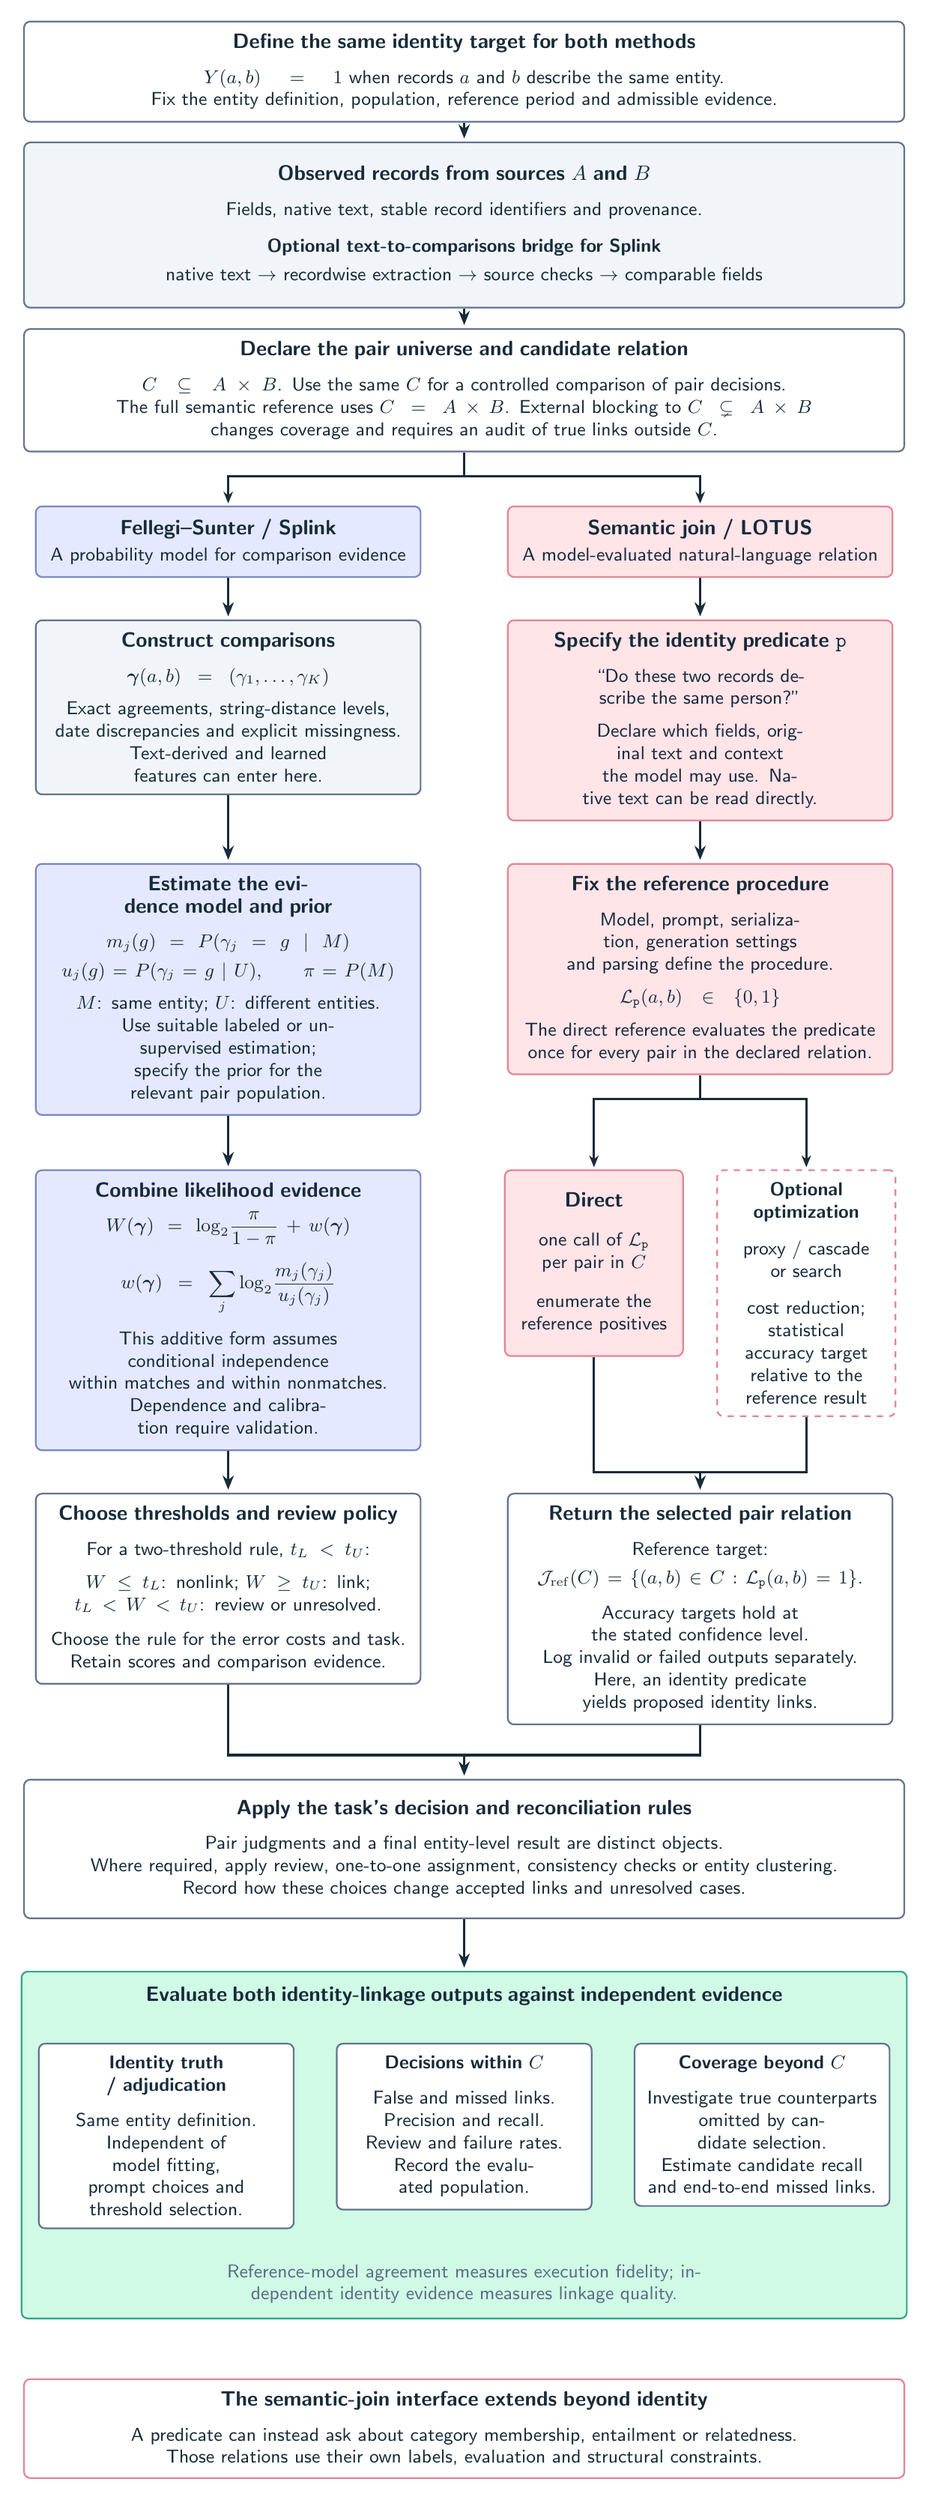
\begin{tikzpicture}[
  every node/.append style={font=\introfont},
  box/.append style={inner sep=6pt,line width=.8pt},
  flow/.append style={line width=1.35pt},
  branch/.append style={line width=1.1pt}
]

\node[box,text width=145mm,minimum height=16mm] (target) at (8,-.75) {\introhead{Define the same identity target for both methods}\\[6pt]
  $Y(a,b)=1$ when records $a$ and $b$ describe the same entity.\\
  Fix the entity definition, population, reference period and admissible evidence.};

\node[data,text width=145mm,minimum height=28mm] (inputs) at (8,-3.35) {\introhead{Observed records from sources $A$ and $B$}\\[6pt]
  Fields, native text, stable record identifiers and provenance.\\[7pt]
  \textbf{Optional text-to-comparisons bridge for Splink}\\[3pt]
  native text $\rightarrow$ recordwise extraction $\rightarrow$ source checks $\rightarrow$ comparable fields};
\draw[flow] (target) -- (inputs);

\node[box,text width=145mm,minimum height=20mm] (candidates) at (8,-6.15) {\introhead{Declare the pair universe and candidate relation}\\[6pt]
  $C\subseteq A\times B$. Use the same $C$ for a controlled comparison of pair decisions.\\
  The full semantic reference uses $C=A\times B$. External blocking to $C\subsetneq A\times B$\\
  changes coverage and requires an audit of true links outside $C$.};
\draw[flow] (inputs) -- (candidates);

\node[model,text width=61mm,minimum height=10mm,anchor=north] (fshead) at ([xshift=-4cm,yshift=-9mm]candidates.south) {\introhead{Fellegi--Sunter / Splink}\\[2pt]A probability model for comparison evidence};
\node[llm,text width=61mm,minimum height=10mm,anchor=north] (semhead) at ([xshift=4cm,yshift=-9mm]candidates.south) {\introhead{Semantic join / LOTUS}\\[2pt]A model-evaluated natural-language relation};
\coordinate (headbus) at ([yshift=-4mm]candidates.south);
\draw[route] (candidates.south) -- (headbus);
\draw[branch] (headbus) -| (fshead.north);
\draw[branch] (headbus) -| (semhead.north);
\node[fit=(fshead)(semhead),inner sep=0pt] (headerrow) {};

\node[data,text width=61mm,minimum height=25mm,anchor=north] (gamma) at ([xshift=-4cm,yshift=-7mm]headerrow.south) {\introhead{Construct comparisons}\\[6pt]
  $\boldsymbol\gamma(a,b)=(\gamma_1,\ldots,\gamma_K)$\\[5pt]
  Exact agreements, string-distance levels,\\
  date discrepancies and explicit missingness.\\
  Text-derived and learned features can enter here.};
\node[llm,text width=61mm,minimum height=25mm,anchor=north] (predicate) at ([xshift=4cm,yshift=-7mm]headerrow.south) {\introhead{Specify the identity predicate $\mathtt p$}\\[6pt]
  ``Do these two records describe the same person?''\\[5pt]
  Declare which fields, original text and context\\
  the model may use. Native text can be read directly.};
\draw[flow] (fshead) -- (gamma);
\draw[flow] (semhead) -- (predicate);
\node[fit=(gamma)(predicate),inner sep=0pt] (rowone) {};

\node[model,text width=61mm,minimum height=30.5mm,anchor=north] (parameters) at ([xshift=-4cm,yshift=-7mm]rowone.south) {\introhead{Estimate the evidence model and prior}\\[6pt]
  $m_j(g)=P(\gamma_j=g\mid M)$\\[3pt]
  $u_j(g)=P(\gamma_j=g\mid U),\qquad \pi=P(M)$\\[5pt]
  $M$: same entity; $U$: different entities.\\
  Use suitable labeled or unsupervised estimation;\\
  specify the prior for the relevant pair population.};
\node[llm,text width=61mm,minimum height=30.5mm,anchor=north] (reference) at ([xshift=4cm,yshift=-7mm]rowone.south) {\introhead{Fix the reference procedure}\\[6pt]
  Model, prompt, serialization, generation settings\\
  and parsing define the procedure.\\[5pt]
  $\mathcal L_{\mathtt p}(a,b)\in\{0,1\}$\\[5pt]
  The direct reference evaluates the predicate\\
  once for every pair in the declared relation.};
\draw[flow] (gamma) -- (parameters);
\draw[flow] (predicate) -- (reference);
\node[fit=(parameters)(reference),inner sep=0pt] (rowtwo) {};

\node[model,text width=61mm,minimum height=31.5mm,anchor=north] (weights) at ([xshift=-4cm,yshift=-9mm]rowtwo.south) {\introhead{Combine likelihood evidence}\\[6pt]
  $W(\boldsymbol\gamma)=\log_2\!\dfrac{\pi}{1-\pi}+w(\boldsymbol\gamma)$\\[7pt]
  $w(\boldsymbol\gamma)=\displaystyle\sum_j\log_2\!\dfrac{m_j(\gamma_j)}{u_j(\gamma_j)}$\\[7pt]
  This additive form assumes conditional independence\\
  within matches and within nonmatches.\\
  Dependence and calibration require validation.};
\draw[flow] (parameters) -- (weights);

\node[llm,text width=26mm,minimum height=31.5mm,anchor=north] (direct) at ([xshift=2.2cm,yshift=-9mm]rowtwo.south) {\introhead{Direct}\\[8pt]
  one call of $\mathcal L_{\mathtt p}$\\
  per pair in $C$\\[8pt]
  enumerate the\\
  reference positives};
\node[box,draw=llmline,dashed,text width=26mm,minimum height=31.5mm,anchor=north] (optimized) at ([xshift=5.8cm,yshift=-9mm]rowtwo.south) {\textbf{Optional\\optimization}\\[7pt]
  proxy / cascade\\
  or search\\[7pt]
  cost reduction;\\
  statistical\\
  accuracy target\\
  relative to the\\
  reference result};
\coordinate (execbus) at ([yshift=-4mm]reference.south);
\draw[route] (reference.south) -- (execbus);
\draw[branch] (execbus) -| (direct.north);
\draw[branch] (execbus) -| (optimized.north);
\node[fit=(weights)(direct)(optimized),inner sep=0pt] (rowthree) {};
\coordinate (rowthreebase) at (candidates.center |- rowthree.south);

\node[box,text width=61mm,minimum height=32mm,anchor=north] (fsdecision) at ([xshift=-4cm,yshift=-7mm]rowthreebase) {\introhead{Choose thresholds and review policy}\\[6pt]
  For a two-threshold rule, $t_L<t_U$:\\[5pt]
  $W\leq t_L$: nonlink; $W\geq t_U$: link;\\
  $t_L<W<t_U$: review or unresolved.\\[6pt]
  Choose the rule for the error costs and task.\\
  Retain scores and comparison evidence.};
\node[box,text width=61mm,minimum height=32mm,anchor=north] (semdecision) at ([xshift=4cm,yshift=-7mm]rowthreebase) {\introhead{Return the selected pair relation}\\[6pt]
  Reference target:\\[3pt]
  $\mathcal J_{\mathrm{ref}}(C)=\{(a,b)\in C:\mathcal L_{\mathtt p}(a,b)=1\}$.\\[6pt]
  Accuracy targets hold at the stated confidence level.\\
  Log invalid or failed outputs separately.\\
  Here, an identity predicate yields proposed identity links.};
\draw[flow] (weights) -- (fsdecision);
\coordinate (semoutbus) at ([yshift=3.5mm]semdecision.north);
\draw[route] (direct.south) |- (semoutbus);
\draw[route] (optimized.south) |- (semoutbus);
\draw[flow] (semoutbus) -- (semdecision.north);
\node[fit=(fsdecision)(semdecision),inner sep=0pt] (rowfour) {};
\coordinate (rowfourbase) at (candidates.center |- rowfour.south);

\node[box,text width=145mm,minimum height=23.5mm,anchor=north] (policy) at ([yshift=-9mm]rowfourbase) {\introhead{Apply the task's decision and reconciliation rules}\\[6pt]
  Pair judgments and a final entity-level result are distinct objects.\\
  Where required, apply review, one-to-one assignment, consistency checks or entity clustering.\\
  Record how these choices change accepted links and unresolved cases.};
\coordinate (policybus) at ([yshift=4mm]policy.north);
\draw[route] (fsdecision.south) |- (policybus);
\draw[route] (semdecision.south) |- (policybus);
\draw[flow] (policybus) -- (policy.north);

\node[title,text width=145mm,anchor=north] (evalhead) at ([yshift=-11mm]policy.south) {\introhead{Evaluate both identity-linkage outputs against independent evidence}};
\node[box,text width=39mm,minimum height=22.5mm,anchor=north] (truthsource) at ([xshift=-5.05cm,yshift=-6mm]evalhead.south) {\textbf{Identity truth / adjudication}\\[6pt]
  Same entity definition.\\
  Independent of model fitting,\\
  prompt choices and\\
  threshold selection.};
\node[box,text width=39mm,minimum height=22.5mm,anchor=north] (pairerror) at ([yshift=-6mm]evalhead.south) {\textbf{Decisions within $C$}\\[6pt]
  False and missed links.\\
  Precision and recall.\\
  Review and failure rates.\\
  Record the evaluated population.};
\node[box,text width=39mm,minimum height=22.5mm,anchor=north] (coverage) at ([xshift=5.05cm,yshift=-6mm]evalhead.south) {\textbf{Coverage beyond $C$}\\[6pt]
  Investigate true counterparts\\
  omitted by candidate selection.\\
  Estimate candidate recall\\
  and end-to-end missed links.};
\node[fit=(truthsource)(pairerror)(coverage),inner sep=0pt] (evalrow) {};
\coordinate (evalrowbase) at (candidates.center |- evalrow.south);
\node[word,text width=139mm,anchor=north] (evalnote) at ([yshift=-5.5mm]evalrowbase) {Reference-model agreement measures execution fidelity; independent identity evidence measures linkage quality.};
\begin{pgfonlayer}{background}
  \node[truth,fit=(evalhead)(truthsource)(pairerror)(coverage)(evalnote),inner sep=6pt] (evaluation) {};
\end{pgfonlayer}
\draw[flow] (policy) -- (evaluation);

\node[box,draw=llmline,text width=145mm,minimum height=16mm,anchor=north] at ([yshift=-10mm]evaluation.south) {\introhead{The semantic-join interface extends beyond identity}\\[6pt]
  A predicate can instead ask about category membership, entailment or relatedness.\\
  Those relations use their own labels, evaluation and structural constraints.};

\end{tikzpicture}
\end{document}
